\documentclass[conference]{IEEEtran}

\IEEEoverridecommandlockouts
% The preceding line is only needed to identify funding in the first footnote. If that is unneeded, please comment it out.
\usepackage{cite}
\usepackage{amsmath,amssymb,amsfonts}
\usepackage{algorithmic}
\usepackage{graphicx}
\usepackage{textcomp}
\usepackage{xcolor}
\usepackage{listings}
\graphicspath{{./images/}}
\def\BibTeX{{\rm B\kern-.05em{\sc i\kern-.025em b}\kern-.08em
    T\kern-.1667em\lower.7ex\hbox{E}\kern-.125emX}}
\begin{document}

\title{Conference Paper Title*\\
{\footnotesize \textsuperscript{*}Note: Sub-titles are not captured in Xplore and
should not be used}
%\thanks{Identify applicable funding agency here. If none, delete this.}
}

\author{\IEEEauthorblockN{1\textsuperscript{st} Given Name Surname}
\IEEEauthorblockA{\textit{dept. name of organization (of Aff.)} \\
\textit{name of organization (of Aff.)}\\
City, Country \\
email address or ORCID}
\and
\IEEEauthorblockN{2\textsuperscript{nd} Given Name Surname}
\IEEEauthorblockA{\textit{dept. name of organization (of Aff.)} \\
\textit{name of organization (of Aff.)}\\
City, Country \\
email address or ORCID}
\and
\IEEEauthorblockN{3\textsuperscript{rd} Given Name Surname}
\IEEEauthorblockA{\textit{dept. name of organization (of Aff.)} \\
\textit{name of organization (of Aff.)}\\
City, Country \\
email address or ORCID}
}

\maketitle

\begin{abstract}
Transacting IoT data must be different in many ways from traditional approaches in order to build much-needed trust in data marketplaces—trust that will be key to their sustainability. Data generated internally to an organization is usually not enough to remain competitive, enhance customer experiences, or improve strategic decision-making. In this paper, we propose a novel approach to construct IoT-enabled data marketplaces via a decentralized and trustless architecture through the posting of trade records while including the transaction process on distributed ledgers. This approach can efficiently enhance the degree of transparency, as all interactions with smart contracts will be written on-chain. Storage via an end-to-end encrypted message channel allows transmitting and accessing trusted data streams over distributed ledgers regardless of the size or cost of the device, while simultaneously making a verifiable Auth-compliant request to the platform. Furthermore, the platform will complete matching, trading and refunding processes without human intervention which also protects the rights of data providers and consumers through a trading policy written on the smart contract.
\end{abstract}

\begin{IEEEkeywords}
privacy computing, crowd sensing, data marketplace, decentralization
\end{IEEEkeywords}

\section{Introduction}
The growth of data marketplaces is an inevitable result of the IoT (Internet of Things) revolution. As physical assets such as ships, factories, vehicles, farms and buildings become digital, their digital twins will gradually act as secure data exchanges.\cite{digitaltwin, AutonomousDriving} As data streams surge across silos and carry value across organizations, traditional value chains will transition into a web of value. This paradigm shift will be more complex to administers, forcing businesses to rethink their competitive play as part of these ecosystems. Data marketplaces will emerge as a means to exchange data, monetize data streams and provide the basis of new business models. We refer to this new wave of value creation, for the Internet of Everything, as the "Economy of Things." There are three main barriers to achieving data marketplace:
\begin{enumerate}
    \item Data owners do not have much control over their data and their data is locked in silos managed by products and services companies.
    \item Data owners only have access to their own data which has little value when it comes to knowledge discovery.
    \item Data owners do not know how to discover knowledge from raw data.
\end{enumerate}

To overcome these barriers, we implemented IoT-enabled data marketplace and sensor data submission functionalities which are intended to be very lightweight and capable of running on embedded devices. They will only need to perform Tangle operations (e.g., producing and consuming secure channels) and communicate with decentralized facilities, which do not rely on single-source network infrastructure. This proposed reference architecture includes functions that could be mapped to different stakeholders, and multiple functions can be implemented by the same administrative stakeholder in a given operational deployment.
\begin{enumerate}
    \item Data Sellers are entities that deploy an IoT infrastructure, for example smart energy meters. These entities are interested in selling the collected data or subsets of that data.
    \item Managed Data Lakes would typically store a massive amount of data and metadata to enable data discovery.
    \item Data Buyers consuming data streams or downloading data sets are interested in the additional value that external data can bring to their internal data.
\end{enumerate}

Looking at Airbox\cite{LASS} as an example, every household with an Airbox device can collect air quality records automatically and autonomically—rather than passively receive the outcomes from the centralized authorities. To protect privacy, data should be encrypted before going on-chain. As for data reliability, we extended the backbone design of the Airbox to interoperate smart-contract-oriented structure to record every transaction. At the same time, data on-chain will send a verifiable request to mark itself as "being tradeable." This step enables buyers to review and bargain at will. Last but not least, payments will be stored on the smart contracts until the transactions are confirmed. The entire sequence is illustrated in Fig.~\ref{fig:airbox}.

\begin{figure}[htbp]
    \centering
    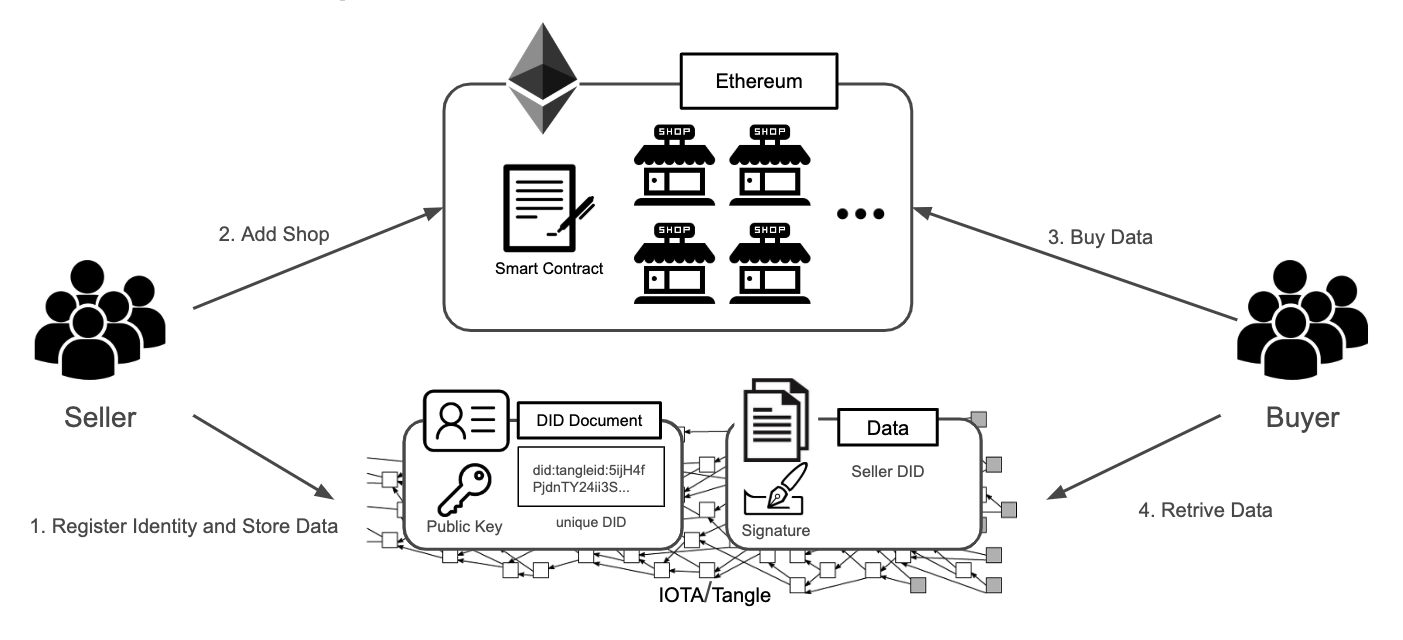
\includegraphics[width=2.5in]{airbox}
    \caption{IoT-enabled personal air quality assistant.}
    \label{fig:airbox}
\end{figure}

Another example is smart meter data which can assist in energy transition. Meanwhile, time smart meter data is privacy-sensitive, that implies power consumption can be associated with appliances used. With measurements every 0.5 seconds, it is possible to determine what television channel is being watched.\cite{SmartGridPrivacy}. Furthermore, by facilitating the aggregate data, the owner of these records can perform the following analysis:
\begin{enumerate}
    \item Detect how many people live at certain house by watching the number of cycles of indoor hot water heater (not accounting for bad hygiene);
    \item Acquaintance with somebody's availability by the energy cycle of the TV;
    \item Know about somebody's activities by the energy signature of the coffee pot or the toaster;
\end{enumerate}

As shown in Fig.~\ref{fig:power_usage}, the data is considered granular data and can be used to track somebody's behavior and location. Once data becomes granular, the "Pandora's box" of data privacy is opened up. Questions such as data ownership, data usage and data protection become new challenges for both utility companies and their infrastructure vendors.

\begin{figure}[htbp]
    \centering
    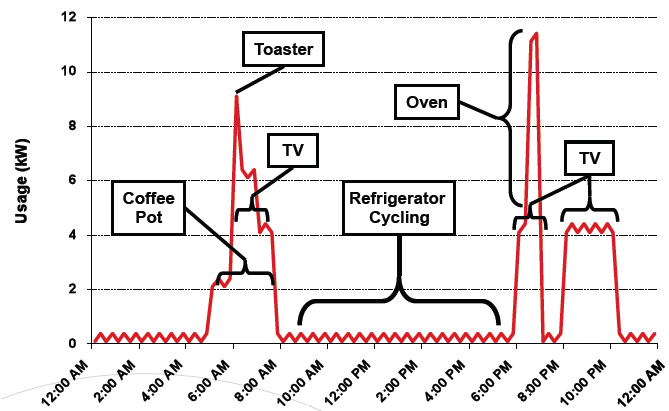
\includegraphics[width=2.5in]{power_usage}
    \caption{Power consumption peaks can be associated with individual appliances. (Source: Privacy Issues Related to Smart Grid Technologies, Megan J. Hertzler)}
    \label{fig:power_usage}
\end{figure}

The General Data Protection Regulation (GDPR) came into effect  May 25, 2018. It provides data and privacy protection for European citizens. When dealing with personal identifiable information (like the measurements of a smart meter) a service provider has to:
\begin{enumerate}
    \item State the goal for data usage clearly (and only use the data for that goal).
    \item Have consent of the consumer to access the data.
    \item Stop collecting data when consent is revoked.
\end{enumerate}

In short, energy usage data cannot be legally shared without adhering to the GDPR. For open usage of smart meter measurements to occur, a solution needs to be provided that adheres to these requirements. Two goals of this solution are: 1) Energy data goes directly from the smart meter to the service provider; 2) Consent (authorizations to access energy data) is stored decentrally. When data or consent is stored centrally, there are privacy concerns. Consent might be irrevocable because a centralized server is down, and it also lead to a vendor lock-in, where the owner of the smart meter data reader determines what service providers can use the data, instead of creating a level playing field where anyone can be authorized to access the data.

The highly flexible value creation networks that result from market economy principles will require new forms of collaboration between companies, depending on the creation of a common global communication and computing infrastructure that allows economic relationships between machines. Our proposed decentralized data marketplace is expected to serve as a vendor and industry-neutral platform, encouraging open innovation and industrial automation.


\section{Related Work}
The publish/subscribe service model consists of publishers, subscribers and brokers, which has been proven\cite{pubSubAnalysis, pubSubAnalysis2} to be an efficient and flexible solution for a large number of diverse entities like IoT applications. A lot of work in publish/subscribe system focused on the scalability and the different security issues such as, encrypted data communication, privacy preserving data subscription and access control of digital asset. A few work targets on the storage which is a vital considerations for IoT and mobile computing and the incentive for data economics.

M. B. Abdullahi and G. Wang\cite{centralPubSub} presented a secure publish/subscribe data storage service in Wireless sensor networks (WSNs) which ensures several security issues. Each user has an identity for authentication, whereas subscribers' interests are encoded before matching to protect users' interests. Additionally, the proposed encryption scheme can prevent adversary to access published data if the sensor node is compromised. However, the access control and encryption keys of data is enforced by the network controllers (NCs) and Cirtificate Authorities (CAs), which may be a potential security risk of the system. Also the storage is not well illustrated in the work. G. S. Ramachandran et al.\cite{trinity} pointed out the security risk of centralized brokers, and applied DLTs to build a distributed pub/sub system which promotes the transparency of interactions of participants and the status of data. With the help of Smart Contract, usesrs can perform data validation easily, and brokers can keep track of data status. But data is plaintext on blockchain, which the privacy problem of sensitive data need to be considered carefully. The economics incentives that can encourage the publishers to participate the system and pay more attention on the quilatiy control are not included. 

In \cite{userCentricData}, the publisher runs a node in blockchain that preserves all the history data of the ledger, therefore, they can publish and manage data without any third-parties. The subscribers request publisher directly and ask them to save a cache space for interested data. The main contribution of the system is to ensure data owners have full controls of produced data, but the data owners need to have well devices and environment to perform such functionalities and preserve data. Also, the rights for accessing digital assets is more compatible in the IoT scenarios instead of copying raw data. Secure Pub-Sub model\cite{SPS}, a brokerless of publish/subscribe model, is proposed to eliminate the security risk of middlewares in the model and to provide a reputation-based fairness payment strategy on blockcahin. The privacy and data security are considered thoroughly with the encryption scheme, while the reputation of publishers, payment and data sharing are deployed on smart contracts that allows all operations are transparent. The reputation system and the punishment rules against malicous acts of subscribers and publishers. Yet, without brokers, providers and subscribers may need to reveal more sensitive information like IP address in order to match the both sides. Another broker-less model in \cite{PrivacyPreservPubSub} protects the subscribers' privacy by encrypting users' interests with the light-weight PKEwET\cite{PKEwET}, which allows publishers to match the subscribers' interests in cipher text. 

Decentralized storage systems allow users to store files in a distributed network that is maintained by individual nodes around the world instead of a central service provider. Nevertheless, DLTs are often used as the backbone of these systems as data storage and also an incentive layer to encourage people get involved in the network. Filecoin \cite{FileCoin} in Inter-Planetary File system(IPFS)\cite{IPFS} is an incentive layer to incent nodes to provide storage. IPFS is a content-based addressing storage model in a peer-to-peer network, which users can obtain the data with the unique hash value through the network. However, no cryptographic system is applied for user-uploaded files. Sia\cite{Sia} splits the uploaded file into multiple data segments encrypted with the owner's private key, then cipher text is sent to the Sia nodes that rent the storage in Siacoin through smart contracts. Files are duplicated in multiple nodes to prevent data loss.
 
\section{System Architecture}
Our proposed data marketplace framework is a 3-tier decentralized architecture with data providers who publish data; data consumers who search for interested products and issue a new trade; and brokers who interact between data providers and consumers, including data publishing, product metadata generation and trading process.

\subsection{Participants}
There are three major roles in the decentralized data marketplace (Fig.~\ref{fig:system_design}).

\begin{itemize}
\item \textbf{Data Provider: }
Data providers, who generate and preserve streaming data, are willing to sell streaming data to consumers and receive subscription fees from consumers, which can be used to improve the quantity and accuracy of their device or service.
\item \textbf{Consumer: }
Consumers aspire to obtain streaming data to promote the value of their service. However, it is a significant challenge for most consumers to collect the desired data by themselves, so they look to purchasing the streaming data from data providers.
\item \textbf{Broker: }
Brokers represent data providers and consumers to perform computing tasks as brokers are expected to have higher resource. Some trustworthy brokers who pass procedures for conformity assessment are added to the decentralized data marketplace. Once a qualified data provider requests to launch a new product, the broker is requested to deal with the trading process and publish the provider’s data streams to the MAM channel. Brokerage fees for each product will be charged by the broker.
\end{itemize}

\begin{figure}[!t]
    \centering
    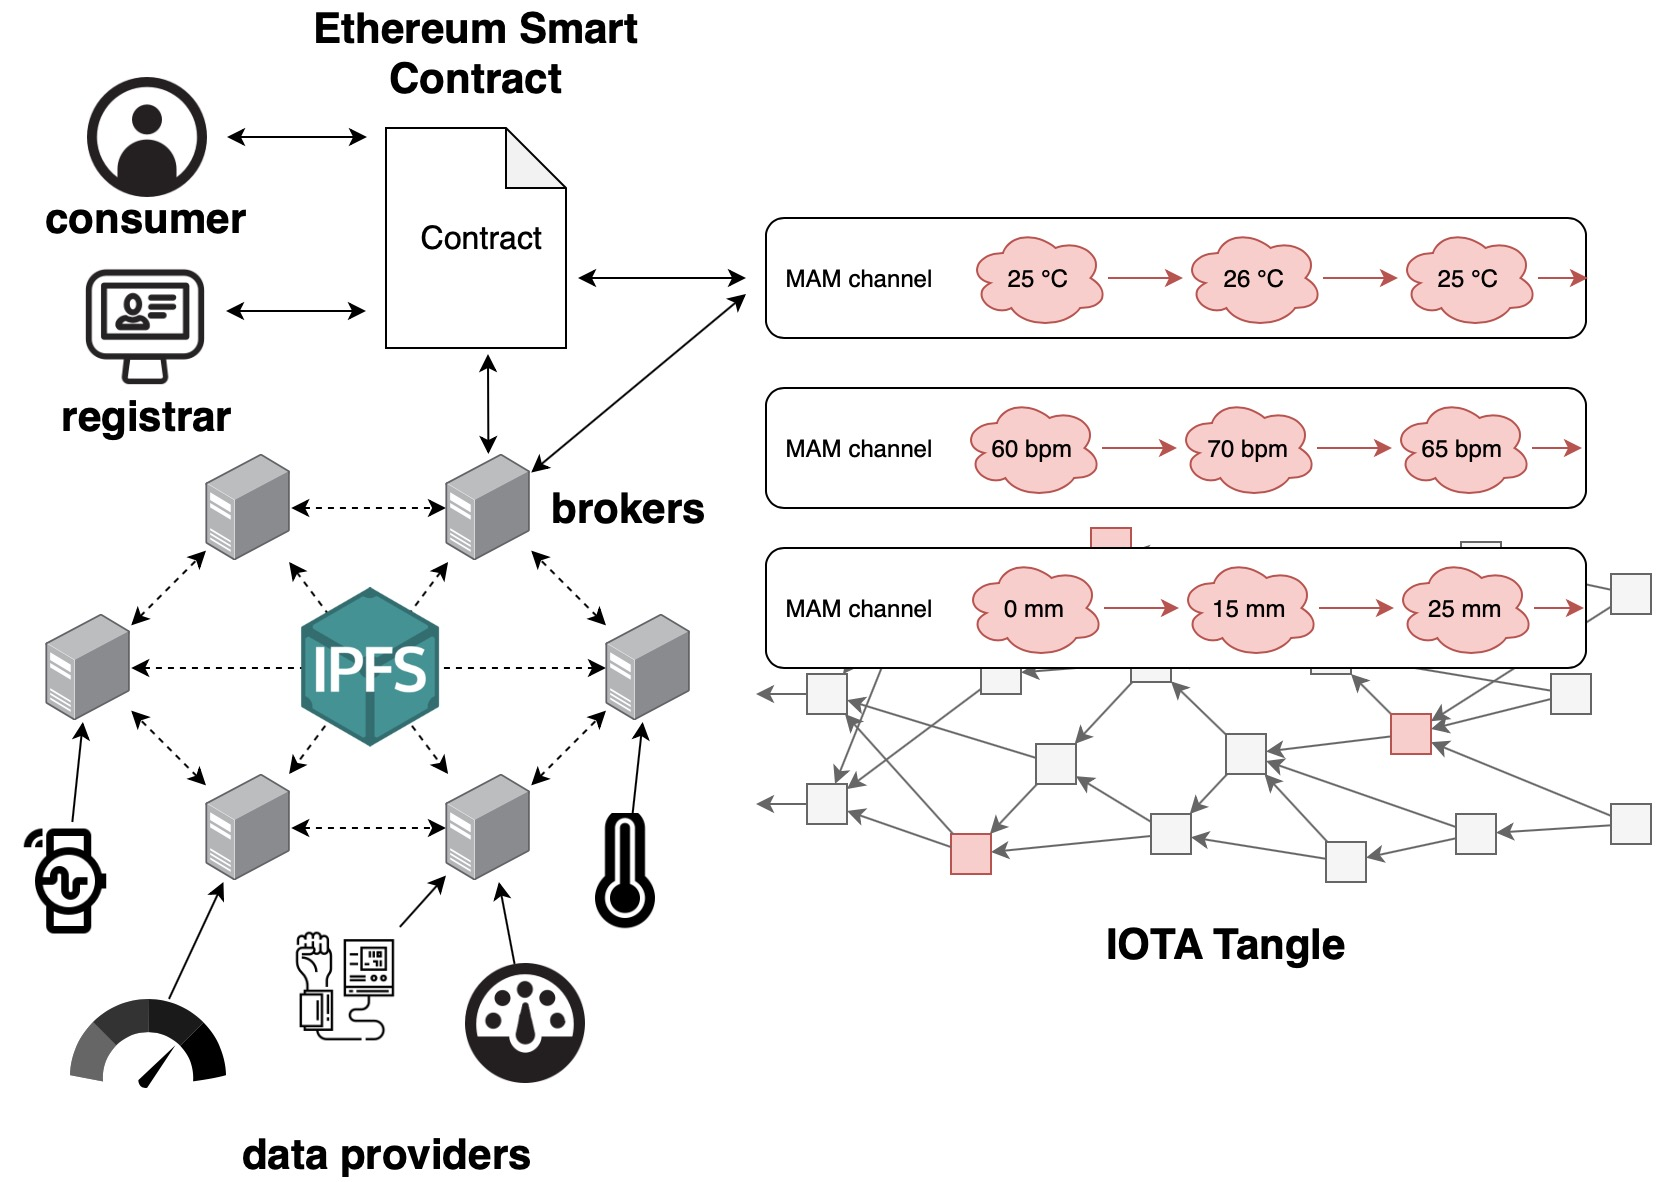
\includegraphics[width=3.5in]{system_design}
    \caption{The system design of a decentralized architecture which consists of data providers, consumers and brokers.}
    \label{fig:system_design}
\end{figure}

\subsection{Components}
There are several building blocks in the proposed design to meet the expectations: 1) emit and access encrypted data stream; 2) retrieve transaction data for audit; 3) digital identity for all participants; and 4) enforcement of transparency and traceability.


\subsubsection{Masked Authenticated Messaging}
IOTA is a feeless cryptocurrency designed for IoT while MAM is the second layer data communication protocol built on top of the IOTA network, the Tangle. MAM resolves the challenge of publishing authenticated streaming data as zero-value transactions to distributed ledgers, and provides the ability to publish and fetch encrypted messages over the Tangle along with data integrity and access control.
With MAM, the rights of accessing data is traded instead of a copy of data itself, which gives a flexibilty for subscribers to obtain data anywhere anywhen that subscribers do not need additional storage to store the data it buy.
 
In the IOTA protocol, seed is the identifier of its owner. An IOTA seed represents the ownership of all things associated with the user in the IOTA ecosystem, such as IOTA tokens or messages on the Tangle. With the seed, the owner can produce addresses and signatures in order to issue transactions or publish messages to MAM channels and endpoints.

Either channel or endpoint is like a singly-linked list. The MAM channel ID and endpoint ID are the addresses of transaction and are the root of a channel and endpoint. Each address of a message can be derived from the previous one. A user can create multiple channels and multiple endpoints under the same channel. The messages can be encrypted with the session key and broadcasted in chronological order to the Tangle by attaching it to an endpoint. This allows only entities that know the session key to be able to decode these messages after retrieving them from the Tangle, and the singly-linked list structure implements the concept of forward secrecy, where anyone has no access to the data back from his/her entry point. Fig.~\ref{fig:mam_struct} shows the architecture of MAM.

\begin{figure}[!t]
    \centering
    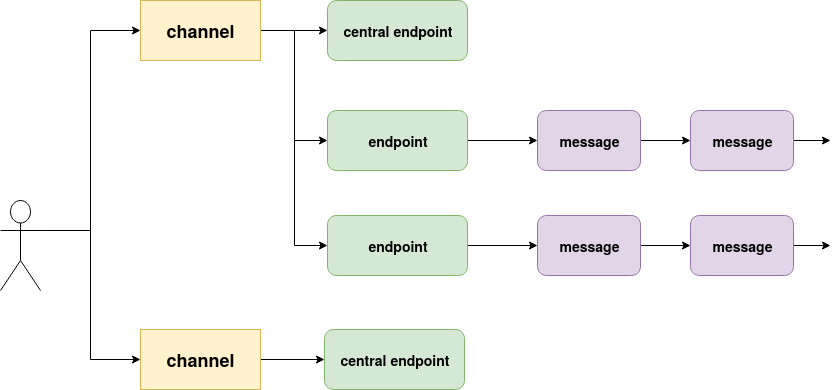
\includegraphics[width=2.5in]{mam_struct}
    \caption{The concept of MAM.}
    \label{fig:mam_struct}
\end{figure}

The authentication in MAM includes source and data authentication. Source authentication ensures that the message originates from the claimed owner, and data authentication ensures the integrity of the data from that sender. These are achieved through the Merkle signature scheme\cite{MSS} (MSS) which is a digital signature scheme based on Merkle Hash Trees and One-way hash functions. However, the size of Merkle Hash Trees should be fixed at start, which is the size of a channel and the endpoint is decided before creation. Thus, data providers need to firstly decide how to distribute data product into MAM channels or endpoints.

%use case illustration
Data providers are the primary role to interact with the MAM. With a seed, a provider can start creating a channel and endpoint. As mentioned above, the length of a channel and an endpoint is fixed, thus providers need to decide the selling unit of data products according to their data type or pricing strategy. Also data providers can a make product preview which is public and not encrypted on MAM. In Fig.~\ref{fig:mam_struct}, a "central endpoint" means its endpoint's ID is the same as channel's ID. By attaching part of the product to central endpoint can give consumers a quick preview with channel's ID only, and users can easily verify the content with digital signatures in messages. Then if the trade is established, providers can then give consumers the encrypted endpoint and session key to consumers.
 
The decentralized and fault-tolerant characteristic of distributed ledgers reduce the risks of centralized storage services, and the underlying IOTA network is scalable which withstands real-time data while increasing users all over the world. Moreover, the features of MAM make it an even better data storage which allows preserving streaming data while ensuring data integrity, proving data ownership to any participants and managing session keys of data. And through the access control and the protocol of MAM, participants are allowed to subscribe to the future data. This ensures that only service requester and selected provider are in possession of a key to decrypt and read the content of the MAM channel and therefore retrieve transaction data for audit.

While the operations of MAM are time-consuming, brokers are responsible not only for being the bridge between providers and consumers, but also for all MAM related operations, such as channel creation and encrypted data publishing in our system. See Fig.~ \ref{fig:launching_product}.

\begin{figure}[!t]
    \centering
    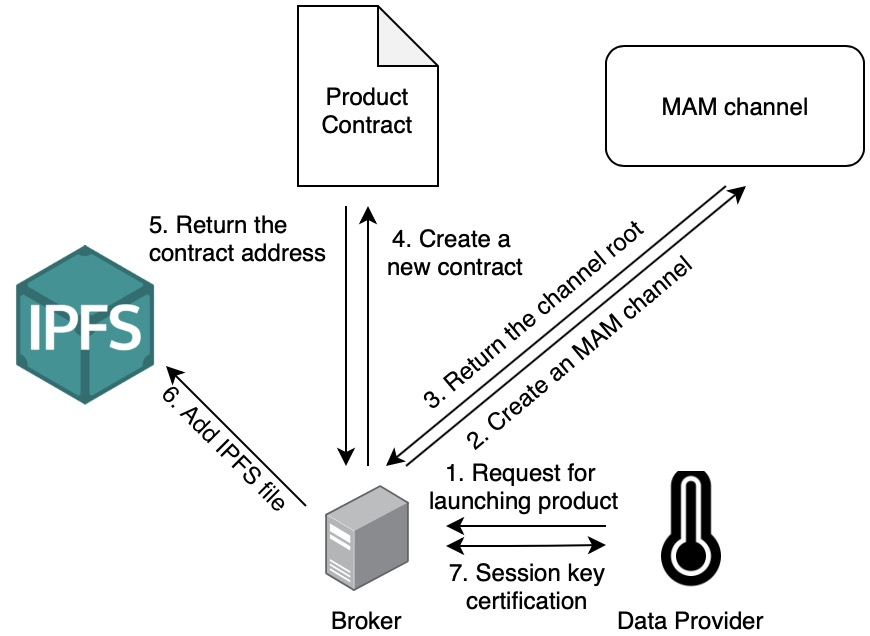
\includegraphics[width=2.5in]{launching_product}
    \caption{The process of launching a product.}
    \label{fig:launching_product}
\end{figure}

\subsubsection{TangleID}
The TangleID\cite{TangleID} is a self-sovereign identity system based on IOTA that does not require any third-party authority to verify an identity and its digital footprint. With TangleID, the digital footprint is converted into digital assets under the principle of Decentralized Identifiers (DIDs)\cite{DID} defined by W3C. Posting DID documents on MAM channel makes TangleID a GDPR-compliant system\cite{GDPR}. Every participant in the data marketplace registers on TangleID, hence one can easily verify data providers' identity to ensure the data persistency from data sources.

A public/private key pair and an IOTA seed are generated in TangleID. The public MAM channel is created with the seed and its MAM channel ID becomes part of the unique user ID, which at the same time serves as DID with the purpose of publishing the public key of the entity. Private key along with the IOTA seed is stored in the local database of the entity. The public/private key pair can be used in secure message sharing within users and digital signature.

The digital identities are also used to establish trust between the communication partners. This is done on two levels to prove that the communication partner owns the DID and the partner can, optionally, proof that it is a trusted participant. This authentication process happens during the first messages of interaction. In order for one partner to listen to another, it authenticates the messages. The DID ownership authentication is done by proving a digitally signed copy of the DID document.

The authentication of trust between the two parties is based on a Verifiable Credential, given out by a trusted issuer for the receiving party. If the receiving party does not trust the issuer, the credential is deemed worthless. If the party is recognized, the credential is verified and the messages will be labelled as trusted. In order to acquire this credential, the party needs to contact the issuer and ask for the credential. The issuer will need to know the DID of the party. If they decide to give out the credential, the issuer will sign the credential and send it encrypted over the blockchain to the requesting party's communication address. This is listed as a Service Endpoint (DID standard) in the DID Document of the requesting party.

\subsubsection{Ethereum Smart Contract}
The smart contract is a protocol for formulating agreement on a blockchain that provides verification and execution of the contract. The code in the smart contract can interact with other contracts, make decisions, store data and transfer cryptocurrency. All conditions and states established in the contract are transparent and enforceable. The appearance of smart contracts makes trading more flexible, and achieves more complex trading patterns in reality.

The Product Contract is used during the trading process, where Product Contract records all the details of data products, such as MAM channel's and endpoint's ID, blinded session key and data providers' DID Document address. Furthermore, data providers and consumers exchange session keys through a Product Contract without involving brokers. Though this design may cost more in transaction fees than doing so off-chain, it is considered a better strategy to assure the profit of both providers and consumers. The further details of key exchangement will be illustrated in Section~\ref{section:trading}.

\subsubsection{Blind Signature}
There is an inherent risk in revealing session keys to brokers since contents may be copied by brokers, which would result in data providers' losses. Therefore, a blind signature is used to prevent session key copying for such circumstances. A blind signature\cite{blindSig} is a form of digital signature where the message is first "blinded" by a random "blinding factor", then passed to a signer to sign. Fig.~\ref{fig:blind_signature} illustrates the steps of blind signature. The resulting message, along with the blinding factor, can be later verified with the signer's public key. In our system design, brokers would perform blind signatures during the process of adding new products for data providers, in order to send the secret key of the MAM channel to the smart contract without knowing it.

\begin{figure}[!t]
	\centering
	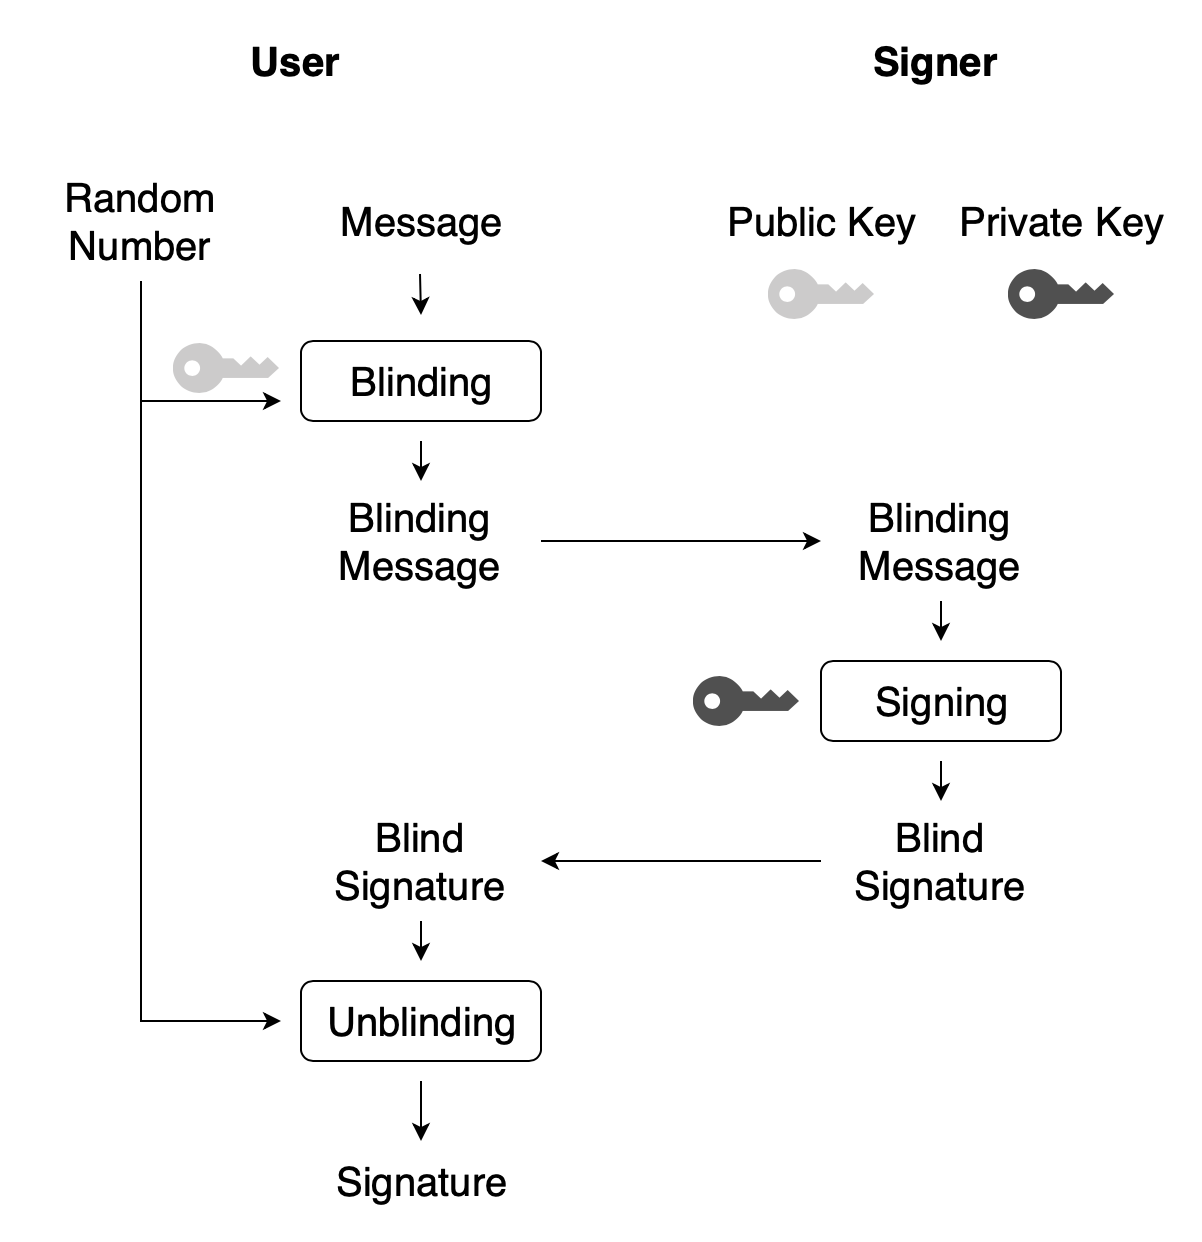
\includegraphics[width=2.5in]{blind_signature}
	\caption{The scheme of blind signature.}
	\label{fig:blind_signature}
\end{figure}

RSA blind signature\cite{cryptoNote} is used in our research. The user chooses a random number $r$ and uses the signer's public key $e$ to generate a blinding factor $r^e$. To prevent the message $m$ from being known by the signer, the user sends blinding message $c$ to the signer instead of $m$.

\begin{equation}
C = r^e m
\end{equation}

The signer signs the blinding message with his private key $d$.

\begin{equation}
S = C^d
\end{equation}

$S$ is the signer's signature of $C$. In RSA system, $ed$ is equal to 1. To remove the blinding factor, the user computes the following calculation.

\begin{equation}
\frac{S}{r}= \frac{C^d}{r} = \frac{(r^e m)^d}{r} = \frac{r^{ed} m^d}{r} = m^d
\end{equation}
 
The user gets $m^d$ which is the signer's signature of the message $m$. At the same time, the signer does not know $m$ and the session key is protected. 

\section{Trading Model}
In the following, we describe the data trading process in detail. To participate a data marketplace, data providers and consumers have to first register on TangleID. Then,  the data provider can launch its product on the marketplace. Once a product is launched, it is searchable and can be subsequently traded. The whole trading and refunding process is defined in smart contracts which are easily traceable and irreversible.

\subsection{Set up}
At the beginning, all participant need to register on TangleID in order to get a DID document and public/private key pairs. The DID document is shared within the following operations to perform authentication, key exchangement and secure communication. 

\subsection{Trading}
\label{section:trading}

The entire trading process is as shown in Fig.~ \ref{fig:trading_product}. Once a consumer wants to subscribe certain streaming data that is generated, he/she has to pay subscription fee to the Product Contract and will be automatically added on the list by the smart contract.

\begin{figure}[!t]
    \centering
    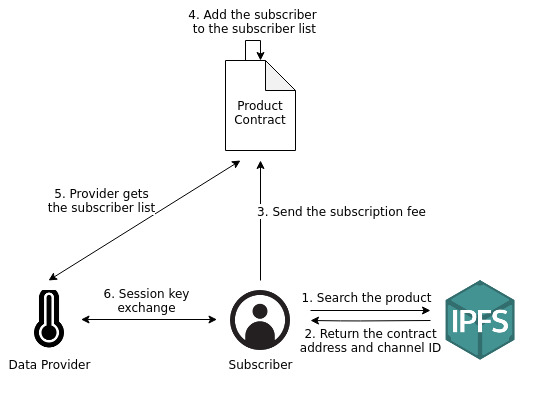
\includegraphics[width=2.5in]{trading_product}
    \caption{The process for the product trading.}
    \label{fig:trading_product}
\end{figure}

Next, session key $k$ should be exchanged between the data provider and consumers. To exchange data, Azaria et al\cite{Medrec} seek an off-chain solution which is based on an end-to-end communication to ensure the efficiency and low costs. However, it is hard to avoid that the data source is unavailable or the sender sends incorrect data intentionally. Instead of using off-chain solution, we use smart contract to transfer the session key\cite{3tierDataMarket} that not only ensures the consistency of the session key, the availability of the source and the traceability of the record, but also prevents malicious participants to cheat others.

\lstdefinestyle{solidity}{
	captionpos=b,
	tabsize=4,
	basicstyle=\scriptsize
}
\lstset{style=solidity}

\begin{lstlisting}[caption={Update encrypt key}, label={lst:key_exchange}, frame=single]
    function addEncryptKey(
        address _consumer,
        string memory _encryptKey
    ) public {
        require(
            msg.sender == provider,
            "Only provider can add blindedKey."
        );
        require(
            consumer2Purchase[_consumer].isKeyAdded == false,
            "One encryptKey has been added."
        );
        consumer2Purchase[_consumer].encryptKey = _encryptKey;
        consumer2Purchase[_consumer].isKeyAdded = true;
        emit newEncryptKey(_consumer, _encryptKey);
    }
\end{lstlisting}

The trading process is shown in Fig.~\ref{fig:key_exchange}. The data provider can obtain public keys of each consumer from the DID document. For each consumer, the data provider encrypts the session key and broker's signature with the consumer's public key and sends the ciphertext $Encrypt(k + Sign(k))$ to the product contract by calling $addEncryptKey()$ (Listing \ref{lst:key_exchange}). Consumers listen to the $newEncryptKey$ event which is triggered when the ciphertext is updated, and decrypt the ciphertext to obtain the session key $k$ and signature $Sign(k)$.

\begin{figure}[!t]
    \centering
    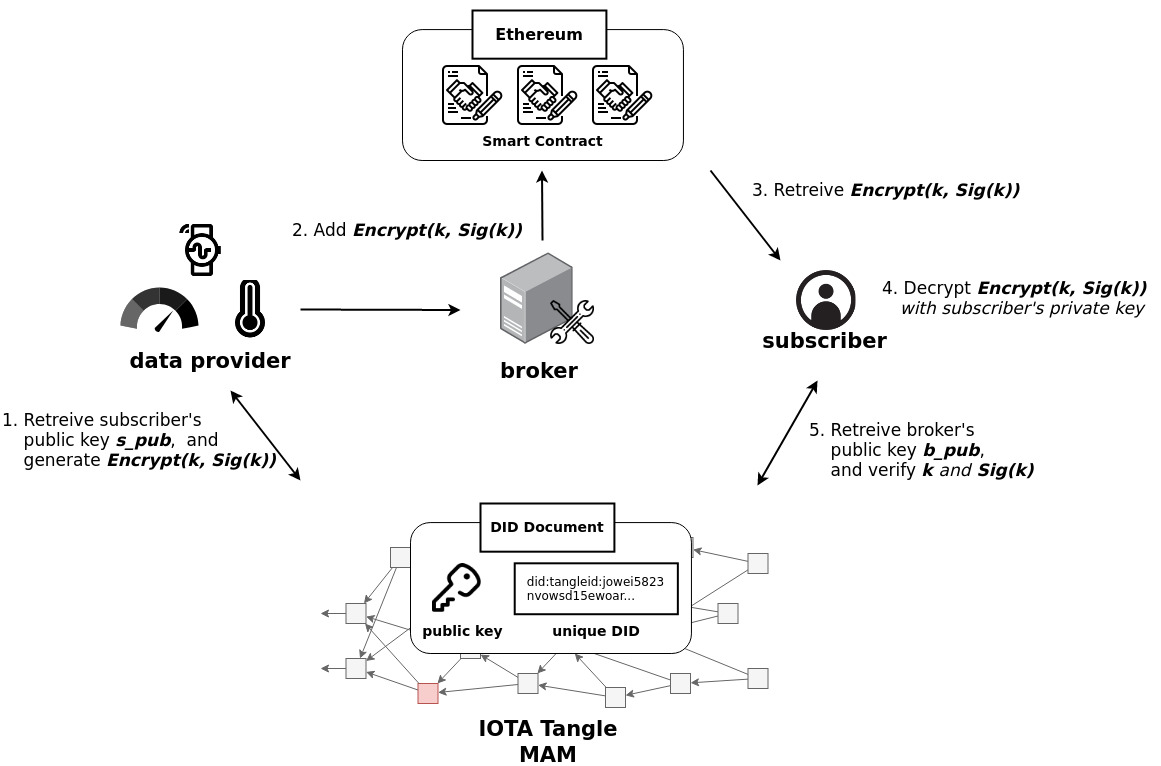
\includegraphics[width=2.5in]{key_exchange}
    \caption{Session key exchange process between the data provider and consumer.}
    \label{fig:key_exchange}
\end{figure}

Consumers can obtain the broker's public key on the DID document as well, so they can verify that the signature is valid and the session key is the only one that is certified by the broker. Afterward, encrypted data is published to the MAM channel, and consumers can obtain and decrypt it with the session key.

\subsection{Refunding}

It is probable that the streaming data sources are delayed or even interrupted after the consumers pay the subscription fee. To protect consumer rights, the subscription fee are not transferred to the data provider until data is generated and published to the MAM channel. If the expected data is not available, consumers can request refunds. We assume that a very small percentage of consumers in the product contract are irrational and/or malicious. When a consumer consents to refund, he can vote at any time. After the ratio of consent votes of refunding is higher than the $threshold$, the subscription fee is proportionally transferred to the data provider, broker and every consumer. Fig.~\ref{fig:refund} shows the refund process.

\begin{figure}[!t]
	\centering
	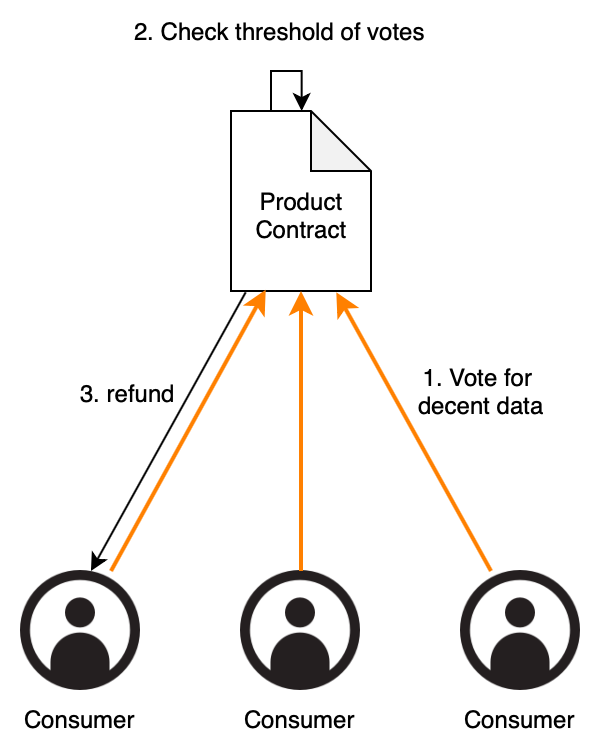
\includegraphics[width=1.5in]{refund}
	\caption{The process of refund.}
	\label{fig:refund}
\end{figure}

The subscription fee can be prorated as below:

\begin{equation}
    F_{DataProvider}(i) = N price \frac{i-1}{M} (1-F_{b}) -F_{t}
\end{equation}

\begin{equation}
    F_{Broker}(i) = N price \frac{i-1}{M} F_{b} -F_{t}
\end{equation}

\begin{equation}
    F_{Consumer}(i) = price \frac{M-i+1}{M} -F_{t}
\end{equation}

where $i$ is the number of data when refunding condition is met, $price$  is the subscription price, $M$ is the number of expected data samples, $F_{b}$ (\%) is the brokerage fee which is expressed as a percentage, $F_{t}$ is the transaction fee of the smart contract, $N$ is the number of consumers in this contract.

To refund or withdraw subscription fees from the smart contract, the data provider, broker, and consumer send a transaction to execute the smart contract and are responsible for the transaction fee. We assume that only a half of the expected records are published to the MAM channel. When $F_{b}$ is 5\%, the data provider and broker can withdraw half of the total subscription fee from the smart contract and 5\% of the subscription fee belongs to the broker while the remaining belongs to the data provider. For consumers, they can receive half of the subscription fee refunded which should be deducted from the transaction fee.

Considering the situation that one of the consumers requests a refund in the future, when the consumer is disappointed with the data quality, he/she may request a refund.

\section{Evaluations}
It is worth making a claim that all participants in data marketplace do not need to hold an IOTA full node which maintains the transaction history and exchanges information of the Tangle. Each role is only required to run client libraries and communicate with IOTA full nodes to interact with the Tangle. Therefore, in the following evaluations, all devices run with client library only.

\subsection{MAM Performance Evaluation}
MAM is a secure and validatable data storage of the proposed architecture. And publishing data to MAM is the primary key to resolve all the difficulties discussed in previous sections. The interactions between data providers and MAM can be frequent. Data providers can either upload data in a short time interval or maintain multiple MAM channels or endpoints at the same time, hence the operation of MAM is one of the bottleneck in data marketplace.

In this section, time measurement is evaluated in two MAM operations: channel/endpoint creation and data attachment to endpoints. To perform the evaluation assessment, a personal computer (PC, 3.2GHz 64-bit 6-core i7-8700 with 16GB DDR4 RAM) and a Raspberry Pi 3 Model B (1.2 GHz 64-bit quad-core ARM Cortex-A53 with 1GB LPDDR2 RAM) have been used to run MAM. 

\subsubsection{Channel / Endpoint Creation}
The length of a channel or endpoint is $2^{height}-1$ where \textit{height} is the height of Merkle Hash Tree in a Merkle signature scheme (MSS), and the "$-1$" is for announcing the ID of next channel or endpoint. A channel with height $n$ can create $2^n-1$ endpoints, and an endpoint with height $m$ can attach $2^m-1$ messages, therefore the capacity of a channel is $2^{nm}-2^n-2^m+1$ messages in total. The greater the \textit{height} of MSS, the longer the channel/endpoint, however the higher the computational power required. In this task, both channel and endpoint creation are tested and the \textit{height} is set from 1 to 7 which is quite enough for data providers to upload data. The results are shown in Table \ref{tab:channel_create} and Table \ref{tab:endpoint_create}. The time duration for each \textit{height} is the average time of running 100 rounds.

\begin{table}[htbp]
	\caption{Time measurement of channel creation}
	\label{tab:channel_create}
	\begin{center}
	\begin{tabular}{|c|c|c|}
	\hline
		\textbf{height of MSS} & \textbf{PC (sec)} & \textbf{Raspberry Pi 3 (sec)} \\ 
		\hline
		1 & 0.26183 & 2.908702 \\ 
		2 & 0.524076 & 5.805524 \\ 
		3 & 1.045942 & 11.555660 \\ 
		4 & 2.092989 & 23.178036 \\ 
		5 & 4.19515 & 46.164079\\ 
		6 & 8.361586 & 92.320173\\ 
		7 & 16.651607 & 185.292243\\
		\hline
	\end{tabular}
	\end{center}
\end{table}

\begin{table}[htbp]
	\caption{Time measurement of endpoint creation}
	\label{tab:endpoint_create}
	\begin{center}
	\begin{tabular}{|c|c|c|}
	\hline
		\textbf{height of MSS} & \textbf{PC (sec)} & \textbf{Raspberry Pi 3 (sec)} \\ 
		\hline
		1 & 0.256425 & 2.887064 \\ 
		2 & 0.505679 & 5.767912 \\ 
		3 & 0.999524 & 11.550455 \\ 
		4 & 1.994017 & 23.260508 \\ 
		5 & 3.965007 & 46.748366 \\ 
		6 & 7.918925 & 93.182975 \\ 
		7 & 16.561419 & 186.064562 \\
		\hline
	\end{tabular}
	\end{center}
\end{table}

The results of Table \ref{tab:channel_create} and Table \ref{tab:endpoint_create} are plotted in Fig.~\ref{fig:mam_create}. Since the creation of channel and endpoint are MSS calculations, the curves of the same hardware are nearly identical. On the other hand, the performance of Raspberry Pi 3 is acceptable when \textit{height} is smaller than 4, but time grows rapidly when \textit{height} is 5 or above. And the performance of PC remains acceptable even \textit{height} gets to 7. The results indicate that MAM channel/endpoint creation is a laborious job for a Raspberry Pi 3 when data providers need a longer channel/endpoint, which is one of the reason that MAM operations should be forwarded to brokers.
  
\begin{figure}[!t]
    \centering
    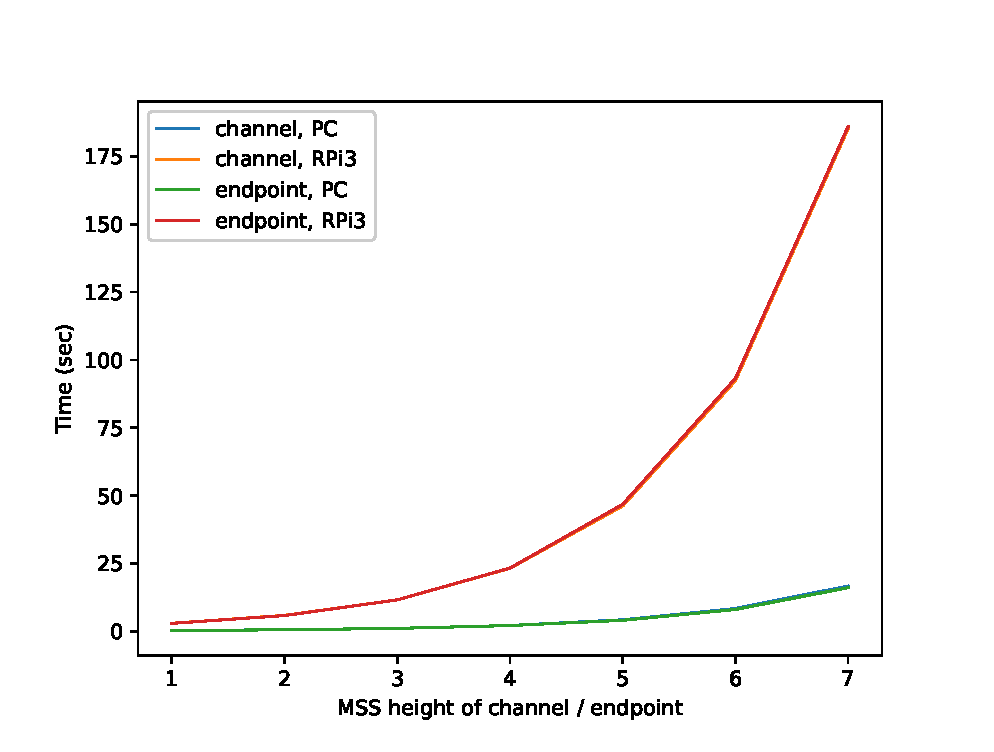
\includegraphics[width=2.5in]{mam_create}
    \caption{Time cost of MAM creation.}
    \label{fig:mam_create}
\end{figure}

\subsubsection{Messages Publishment}
Publishing a message to MAM is attaching a zero-value transaction to the Tangle which requires two processes:
\begin{itemize}
	\item	Tips selection: In the IOTA protocol, a new-coming transaction needs to pick up 2 existed transactions called tips to reference and verify. The tips are provided by IOTA full nodes.
	\item	Proof-of-Work (PoW): An algorithm which prevents Denial of Service and spam attacks on a network. a computationally hard puzzle to solve, but easy to verify. IOTA uses a Hashcash\cite{Hashcash} based puzzle.
\end{itemize}

Tips selection requires a stable network connection to wait the response from IOTA full nodes, and PoW requires enough computation resources to perform. Fig.~\ref{fig:mam_send} shows PDF of publishing one message to MAM endpoint for 100 times. The average time for PC to send a message is 48.1069 seconds, and Raspberry Pi 3 takes 743.8586 seconds.

\begin{figure}[!t]
    \centering
    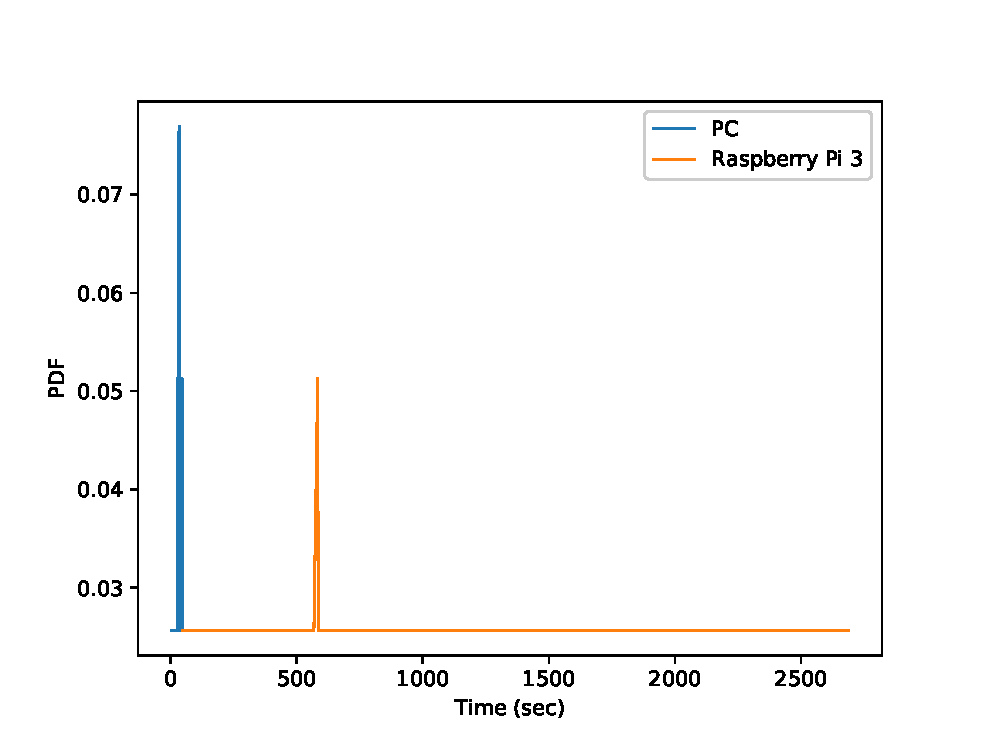
\includegraphics[width=2.5in]{mam_send}
    \caption{Time cost of sending a message through MAM.}
    \label{fig:mam_send}
\end{figure}

MAM operations take a lot of time for both devices, but Raspberry Pi 3 spends even more time than PC. The simulation results above indicate that MAM is difficult for low-level sensor devices to run, which these devices are the majority hardware as data providers in the data marketplace. Furthermore, sensors with the low computing power and weak internet connection are not able to have enough resources to handle data collection, data transmission on MAM and trading process with consumers simultaneously. 

Therefore, transferring MAM operations to brokers while ensuring the profit and privacy of providers through blind signatures can effectively solve performance problems and lower the threshold for participation in the data marketplace. Brokers can be PCs or powerful machines that runs Ethereum client and Tangle-accelerator\cite{TA}. Where Ethereum client is used to interact with Ethereum and Tangle-accelerator is a caching proxy server for IOTA, which can serve thousands of IOTA requests at once without accessing remote IOTA full nodes frequently and provide PoW acceleration. Fig.~ \ref{fig:ta_struct} shows the structure of Tangle-accelerator. However, MAM operations still cost a considerable time, improving the performance of MAM is an essential issue that needs to be done for the next step.  

\begin{figure}[!t]
    \centering
    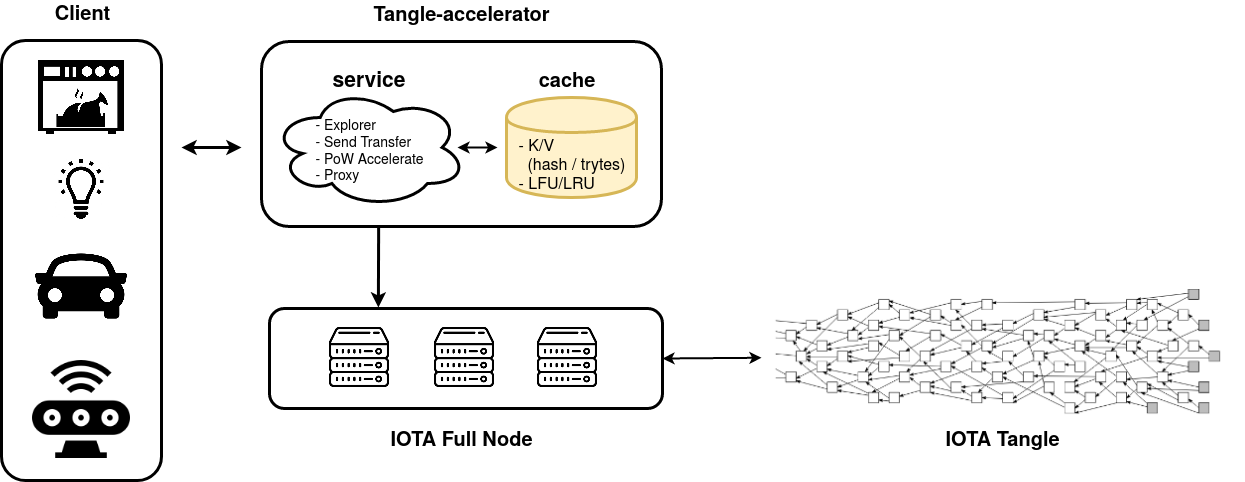
\includegraphics[width=2.5in]{ta_structure}
    \caption{The structure of Tangle-accelerator.}
    \label{fig:ta_struct}
\end{figure}

\section{Conclusions}
By combining the established standards and openly-developed specifications, this paper proposed an autonomous data marketplace design to serve as a vendor and industry-neutral platform, automating the trading of digital assets and services. It was built with blockchain network, immutable audit trails, and contracts with an integrated decentralized identity system, to ensure the authenticity of all participants and enable secure communication and flexible trading mechanisms.

%\section*{Acknowledgment}

\bibliographystyle{IEEEtran}
\bibliography{references}

\end{document}
